\dev{Emile Martinez}{livre de bob, cormen (pour la question à la fin)}

\begin{definition}
	\textbf{3-SAT} : $\varphi = \bigwedge\limits_{i=1}^p C_i$ avec $C_i = l_{i,1} \vee l_{i,2} \vee l_{i,3}$ ($l_{i,j} \in \{x_1, \dots, x_n, \overline{x_1}, \dots, \overline{x_n}\}$)\\ est-elle satisfiable ?
\end{definition}

\begin{com}
	$l$ c'est pour litéral
\end{com}

\begin{enumerate}
	\item 3-SAT $\in$ NP \\
	$\to$ On prend comme certificat la valuation qui met $\varphi$ à vrai (bien polynomial)
	
	\item Reduction deuis SAT-FNC

	\begin{definition}
		\textbf{SAT-FNC} : $\varphi = \bigwedge\limits_{i=1}^p C_i$ avec $C_i = \bigvee\limits_{j=1}^{k_i} l_{i,j}$ ($l_{i,j} \in \{x_1, \dots, x_n, \overline{x_1}, \dots, \overline{x_n}\}$)\\ est-elle satisfiable ?
	\end{definition}

	SAT-FNC est bien NP-complet.
	
	\item Soit $\varphi$ une instance de SAT-FNC.\\
	Transformons la en une instance de 3-SAT.\\
	
	Soit $i\in \llbracket 1, p\rrbracket$
	\begin{itemize}[label=$\star$]
		\item Si $k_i = 1$, on pose $C_i' = l_{i,1} \vee l_{i,1} \vee l_{i,1}$
		\item Si $k_i = 2$, on pose $C_i' = l_{i,1} \vee l_{i, 2} \vee l_{i,2}$
		\item Si $k_i = 3$, on pose $C_i' = C_i$
		\item Si $k_i \geq 4$, on prend alors de nouvelles variables $y_{i,j}$
		On pose alors $$\begin{array}{rl}
			C_i' = & l_{i,1} \vee l_{i,2} \vee y_{i,2} \\
			\wedge & \bigwedge\limits_{j = 3}^{k_i - 2} \overline{y_{i, j-1}} \vee l_{i,j} \vee y_{i,j}\\
			\wedge & \overline{y_{i, k_i-2}} \vee l_{i, k_i-1} \vee l_{i, k_i}
		\end{array}$$
		\begin{com}
			Expliquer ici que quand un $l_{i,j}$ sera a vrai, on pourra vérfier toutes celles au dessus avec des y à 1, et toutes celles en dessous avec des y à 0. Peut etre que ca serait plus clair en ecrivant la formule avec des pointillées, mais c'est plus long et moins formel. On pourrait faire les deux, mais a voir le temps
		\end{com}
	\end{itemize}
	On prend alors $\varphi' = \bigwedge\limits_{i=1}^p C_i'$ qui est une instance de 3-SAT.\\
	\begin{rem}
		$C_i'$ ici sont des conjonctions de clauses de taille 3.
	\end{rem}

	Pour chaque clause, on a rajouter au plus $k_i$ variables et chaque nouvelle variable apparaît au plus 2 fois, chaque ancienne apparait au plus 3 fois plus (pour $k_i = 1$). Donc notre transformation $\varphi \rightsquigarrow \varphi'$ est polynomiale.
	
	\item Montrons que $\varphi \in \text{SAT-FNC} \Leftrightarrow \varphi' \in \text{3-SAT}$
	\begin{com}
		Différent de $\varphi \leftrightarrow \varphi'$
	\end{com}
	
	$\boxed{\Rightarrow}$ Supposons $\varphi \in \text{SAT-FNC}$.\\
	Alors $\exists \sigma : V \to \{0,1\} : [\varphi]_\sigma = 1$.\\
	Pour chaque $C_i$, on choisit $n_i \in \llbracket 1, k_i \rrbracket$ tel que $[l_{i, n_i}]_\sigma = 1$.\\
	On pose alors $\sigma'(x) = \left\{ \begin{array}{ll}
		1 & \text{si } x = y_{i,j} \text{ avec } j < m_i\\
		0 & \text{si } x = y_{i,j} \text{ avec } j \geq m_i\\
		\sigma(x) & \text{sinon}
	\end{array} \right.$\\
	
	Montrons alors que $[C_i']_\sigma = 1$ : \begin{itemize}[label = $\star$]
		\item Si $k_i \leq 3$, c'est immédiat
		\item Sinon, \begin{itemize}[label=$\bullet$]
			\item $\forall j < n_i, \, \left[ \overline{y_{i, j-1}} \vee l_{i,j} \vee y_{i,j} \right]_{\sigma'} = 1$ car $\sigma'(y_{i,j}) = 1$
			\item $\left[ \overline{y_{i, n_i-1}} \vee l_{i,n_i} \vee y_{i,n_i} \right]_{\sigma'} = 1$ car $ \left[ l_{i,n_i} \right]_{\sigma'} = 1$ (choix de $n_i$ et définition de $\sigma'$)
			\item $\forall j > n_i, \left[ \overline{y_{i, j-1}} \vee l_{i,j} \vee y_{i,j} \right]_{\sigma'} = 1$ car $\sigma'(y_{i, j-1}) = 0$ 
			\item Pareil pour les clauses extrémales.
		\end{itemize}
	\end{itemize}\enspace \\
	
	$\boxed{\Leftarrow}$ Supposons $\varphi' \in \text{3-SAT}$.\\
	
	$\exists \sigma : V \to \{0,1\} : [\varphi']_\sigma = 1$.\\
	Alors $[\varphi]_\sigma = 1$.\\
	\hspace*{1cm}Idée de la preuve : si ce n'est pas le cas, on a $[c_i]_\sigma = 0$.
	
	\hspace*{1cm}Alors comme $[C_i']_\sigma = 1$, on a $\sigma(y_{i, 2}) = 1$ donc $\sigma(y_{i, 3}) = 1$, etc.
	
	\hspace*{1cm}Tous les $y_{i,j}$ sont donc à vrai, donc $\left[\overline{y_{i, k_i-2}} \vee l_{i, k_i-1} \vee l_{i, k_i}\right]_\sigma = 0 $ donc $\left[\varphi'\right]_\sigma = 0$

\end{enumerate}

Ainsi, 3-SAT est NP-complet.

\begin{com}
	Ce qui suit n'est à faire que suivant le temps
\end{com}

\paragraph{Question} Peut-on réduire directement depuis $SAT$ ?¨ \\
\begin{minipage}{0.5\linewidth}
	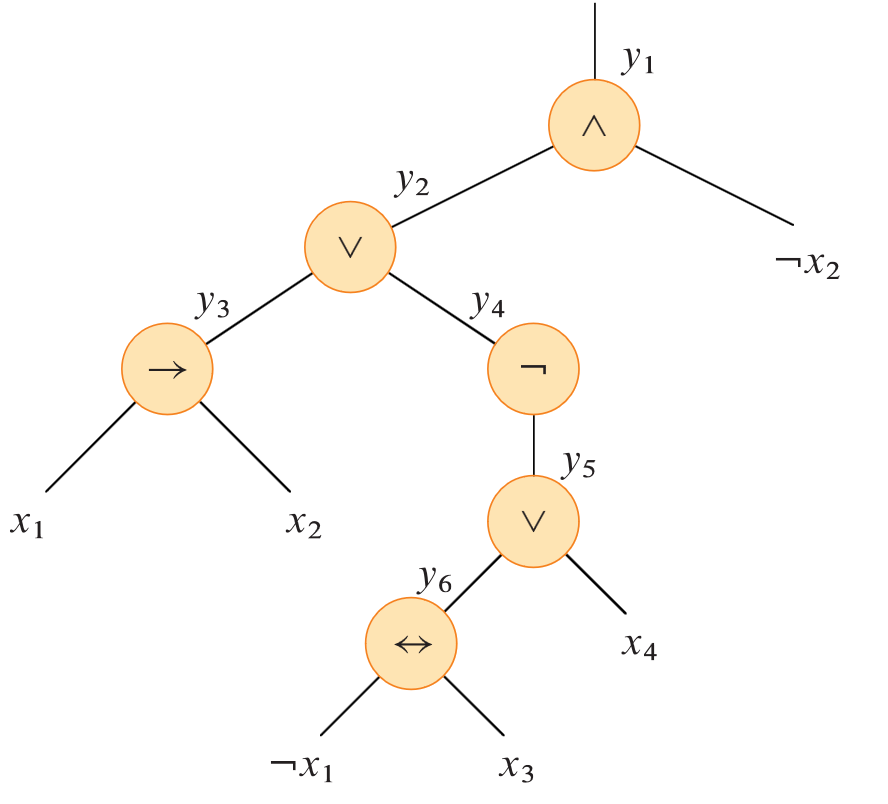
\includegraphics[width = \linewidth]{Developpements/3 SAT/exemple_formule_cormen.png}
\end{minipage}\begin{minipage}{0.5\linewidth}
	Cette arbre représente la formule $$ \varphi \: = \: ((x_1 \to x_2) \vee \neg  ((\neg x_1 \leftrightarrow x_3) \vee x_4)) \wedge \neg x_2$$
	On met alors une variable par sommet, et on transforme en la formule suivante :
	$$\begin{array}{rl}
		\varphi' \: = \: y_1 \enspace \wedge & (y_1 \leftrightarrow (y_2 \wedge \neg x_2))\\
		\wedge & (y_2 \leftrightarrow (y_3 \vee y_4))\\
		\wedge & (y_3 \leftrightarrow (x_1 \to x_2)) \\
		\wedge & (y_4 \leftrightarrow \neg y_5) \\
		\wedge & (y_5 \leftrightarrow (y_6 \vee x_4))\\
		\wedge & (y_6 \leftrightarrow (\neg x_1 \leftrightarrow x_3))
	\end{array}$$
\end{minipage}
